\section{Results}
\label{sec:results}
% TODO: Success vs. corridor length beyond the context window,
% ablations (memory layer, top-k, gate, stop-grad), compute cost.
% TODO: interpret the tables and figures below.
% refs: \cite{esslinger2022dtqn,wu2022memorizing,agarwal2021rliable}

All agents are trained on the Passive T-Maze with corridor length 10, so the cue
is 11 observations before the decision, for 32\,000 training steps after 50\,000
prefill steps, with five training seeds per configuration. DTQN and DTQN-kNN use
contexts of 6 (beyond the window) and 12 (within it) with 2 or 3 transformer
layers; DRQN uses training sequences of 6, 12 and 18 steps; memoryless DQN is a
lower bound. Each run is evaluated greedily on 100 episodes every 2\,000 training
steps; the evaluation seed is $10\,000$ plus the training seed, so runs do not
share evaluation episodes. Scores are final success rates and final returns
min-max normalized per task, aggregated over seeds with stratified bootstrap
confidence intervals (50\,000 replications) \cite{agarwal2021rliable}. All 60
runs used the same source code on one GPU.

Table~\ref{tab:hypothesis-criteria} applies the criteria of
Section~\ref{sec:experimental-setup}. For DTQN-kNN with context 6 and 3 layers,
the IQM point estimate meets the target while the lower bound of its 95\%
confidence interval is 0.67 (Table~\ref{tab:aggregate-metrics}): one of the five
seeds reached 51\% success without a fixed-side policy.

\begin{table}[t]
\centering
\small
\caption{Hypothesis criteria for each DTQN-kNN/DTQN pair with the same context length and number of layers. Beyond the window: an IQM success rate of at least 0.9 and the 95\% CI of P(candidate > baseline) above 0.5. Within the window: that CI not entirely below 0.5 and an IQM at most 0.05 below the baseline (non-inferiority).}
\label{tab:hypothesis-criteria}
\resizebox{\ifdim\width>\linewidth\linewidth\else\width\fi}{!}{%
\begin{tabular}{lrrrrrr}
\toprule
candidate & baseline & regime & candidate IQM & baseline IQM & P(candidate > baseline) & met \\
\midrule
DTQN-kNN context=6 layers=2 & DTQN context=6 layers=2 & beyond window & 1.0 & 0.48 & 1.00 [1.00, 1.00] & yes \\
DTQN-kNN context=6 layers=3 & DTQN context=6 layers=3 & beyond window & 1.0 & 0.48 & 0.94 [0.76, 1.00] & yes \\
DTQN-kNN context=12 layers=2 & DTQN context=12 layers=2 & within window & 1.0 & 1.0 & 0.50 [0.50, 0.50] & yes \\
DTQN-kNN context=12 layers=3 & DTQN context=12 layers=3 & within window & 1.0 & 1.0 & 0.50 [0.50, 0.50] & yes \\
\bottomrule
\end{tabular}}
\end{table}

\begin{table}[t]
\centering
\small
\caption{Final success rate over training seeds: point estimate, 95\% stratified bootstrap confidence interval and standard deviation over runs.}
\label{tab:aggregate-metrics}
\resizebox{\ifdim\width>\linewidth\linewidth\else\width\fi}{!}{%
\begin{tabular}{lrrrrr}
\toprule
algorithm & Mean & IQM & Median & Optimality Gap & Std \\
\midrule
DQN context=1 layers=2 & 0.46 [0.42, 0.49] & 0.47 [0.41, 0.50] & 0.46 [0.42, 0.49] & 0.54 [0.51, 0.58] & 0.043 \\
DRQN context=6 layers=2 & 0.47 [0.43, 0.51] & 0.48 [0.41, 0.52] & 0.47 [0.43, 0.51] & 0.53 [0.49, 0.57] & 0.054 \\
DTQN context=6 layers=2 & 0.47 [0.43, 0.51] & 0.48 [0.41, 0.52] & 0.47 [0.43, 0.51] & 0.53 [0.49, 0.57] & 0.054 \\
DTQN-kNN context=6 layers=2 & 1.00 [1.00, 1.00] & 1.00 [1.00, 1.00] & 1.00 [1.00, 1.00] & 0.00 [0.00, 0.00] & 0.0 \\
DTQN context=6 layers=3 & 0.47 [0.43, 0.51] & 0.48 [0.41, 0.52] & 0.47 [0.43, 0.51] & 0.53 [0.49, 0.57] & 0.054 \\
DTQN-kNN context=6 layers=3 & 0.90 [0.71, 1.00] & 1.00 [0.67, 1.00] & 0.90 [0.71, 1.00] & 0.10 [0.00, 0.29] & 0.219 \\
DRQN context=12 layers=2 & 1.00 [1.00, 1.00] & 1.00 [1.00, 1.00] & 1.00 [1.00, 1.00] & 0.00 [0.00, 0.00] & 0.0 \\
DTQN context=12 layers=2 & 1.00 [1.00, 1.00] & 1.00 [1.00, 1.00] & 1.00 [1.00, 1.00] & 0.00 [0.00, 0.00] & 0.0 \\
DTQN-kNN context=12 layers=2 & 1.00 [1.00, 1.00] & 1.00 [1.00, 1.00] & 1.00 [1.00, 1.00] & 0.00 [0.00, 0.00] & 0.0 \\
DTQN context=12 layers=3 & 1.00 [1.00, 1.00] & 1.00 [1.00, 1.00] & 1.00 [1.00, 1.00] & 0.00 [0.00, 0.00] & 0.0 \\
DTQN-kNN context=12 layers=3 & 1.00 [1.00, 1.00] & 1.00 [1.00, 1.00] & 1.00 [1.00, 1.00] & 0.00 [0.00, 0.00] & 0.0 \\
DRQN context=18 layers=2 & 1.00 [1.00, 1.00] & 1.00 [1.00, 1.00] & 1.00 [1.00, 1.00] & 0.00 [0.00, 0.00] & 0.0 \\
\bottomrule
\end{tabular}}
\end{table}

\begin{table}[t]
\centering
\small
\caption{Probability that a run of the candidate beats a run of the baseline on the same task, with 95\% bootstrap confidence interval.}
\label{tab:probability-of-improvement}
\resizebox{\ifdim\width>\linewidth\linewidth\else\width\fi}{!}{%
\begin{tabular}{lrr}
\toprule
candidate & baseline & P(candidate > baseline) \\
\midrule
DTQN-kNN context=6 layers=2 & DTQN context=6 layers=2 & 1.00 [1.00, 1.00] \\
DTQN-kNN context=6 layers=3 & DTQN context=6 layers=3 & 0.94 [0.76, 1.00] \\
DTQN-kNN context=12 layers=2 & DTQN context=12 layers=2 & 0.50 [0.50, 0.50] \\
DTQN-kNN context=12 layers=3 & DTQN context=12 layers=3 & 0.50 [0.50, 0.50] \\
DTQN-kNN context=6 layers=2 & DRQN context=6 layers=2 & 1.00 [1.00, 1.00] \\
DTQN-kNN context=12 layers=2 & DRQN context=12 layers=2 & 0.50 [0.50, 0.50] \\
DTQN context=6 layers=2 & DRQN context=6 layers=2 & 0.50 [0.14, 0.86] \\
DTQN context=12 layers=2 & DRQN context=12 layers=2 & 0.50 [0.50, 0.50] \\
\bottomrule
\end{tabular}}
\end{table}

\begin{table}[t]
\centering
\small
\caption{Final return, min-max normalized per task over all runs: point estimate, 95\% stratified bootstrap confidence interval and standard deviation.}
\label{tab:aggregate-metrics-return}
\resizebox{\ifdim\width>\linewidth\linewidth\else\width\fi}{!}{%
\begin{tabular}{lrrrrr}
\toprule
algorithm & Mean & IQM & Median & Optimality Gap & Std \\
\midrule
DQN context=1 layers=2 & 0.72 [0.70, 0.74] & 0.73 [0.70, 0.74] & 0.72 [0.70, 0.74] & 0.28 [0.26, 0.30] & 0.022 \\
DRQN context=6 layers=2 & 0.73 [0.71, 0.75] & 0.73 [0.70, 0.75] & 0.73 [0.71, 0.75] & 0.27 [0.25, 0.29] & 0.027 \\
DTQN context=6 layers=2 & 0.73 [0.71, 0.75] & 0.73 [0.70, 0.75] & 0.73 [0.71, 0.75] & 0.27 [0.25, 0.29] & 0.027 \\
DTQN-kNN context=6 layers=2 & 1.00 [1.00, 1.00] & 1.00 [1.00, 1.00] & 1.00 [1.00, 1.00] & 0.00 [0.00, 0.00] & 0.0 \\
DTQN context=6 layers=3 & 0.73 [0.71, 0.75] & 0.73 [0.70, 0.75] & 0.73 [0.71, 0.75] & 0.27 [0.25, 0.29] & 0.027 \\
DTQN-kNN context=6 layers=3 & 0.94 [0.82, 1.00] & 1.00 [0.80, 1.00] & 0.94 [0.82, 1.00] & 0.06 [0.00, 0.18] & 0.135 \\
DRQN context=12 layers=2 & 1.00 [1.00, 1.00] & 1.00 [1.00, 1.00] & 1.00 [1.00, 1.00] & 0.00 [0.00, 0.00] & 0.0 \\
DTQN context=12 layers=2 & 1.00 [1.00, 1.00] & 1.00 [1.00, 1.00] & 1.00 [1.00, 1.00] & 0.00 [0.00, 0.00] & 0.0 \\
DTQN-kNN context=12 layers=2 & 1.00 [1.00, 1.00] & 1.00 [1.00, 1.00] & 1.00 [1.00, 1.00] & 0.00 [0.00, 0.00] & 0.0 \\
DTQN context=12 layers=3 & 1.00 [1.00, 1.00] & 1.00 [1.00, 1.00] & 1.00 [1.00, 1.00] & 0.00 [0.00, 0.00] & 0.0 \\
DTQN-kNN context=12 layers=3 & 1.00 [1.00, 1.00] & 1.00 [1.00, 1.00] & 1.00 [1.00, 1.00] & 0.00 [0.00, 0.00] & 0.0 \\
DRQN context=18 layers=2 & 1.00 [1.00, 1.00] & 1.00 [1.00, 1.00] & 1.00 [1.00, 1.00] & 0.00 [0.00, 0.00] & 0.0 \\
\bottomrule
\end{tabular}}
\end{table}

\begin{table}[t]
\centering
\small
\caption{Runs whose final evaluation ends in the same branch in more than 90\% of episodes (fixed-side policies), and mean final success rate.}
\label{tab:side-bias-summary}
\resizebox{\ifdim\width>\linewidth\linewidth\else\width\fi}{!}{%
\begin{tabular}{lrrr}
\toprule
algorithm & task & fixed-side runs & mean success rate \\
\midrule
DQN context=1 layers=2 & env=PassiveTMaze-v0 corridor\_length=10 & 5/5 & 0.46 \\
DRQN context=6 layers=2 & env=PassiveTMaze-v0 corridor\_length=10 & 5/5 & 0.472 \\
DRQN context=12 layers=2 & env=PassiveTMaze-v0 corridor\_length=10 & 0/5 & 1.0 \\
DRQN context=18 layers=2 & env=PassiveTMaze-v0 corridor\_length=10 & 0/5 & 1.0 \\
DTQN context=6 layers=2 & env=PassiveTMaze-v0 corridor\_length=10 & 5/5 & 0.472 \\
DTQN context=6 layers=3 & env=PassiveTMaze-v0 corridor\_length=10 & 5/5 & 0.472 \\
DTQN context=12 layers=2 & env=PassiveTMaze-v0 corridor\_length=10 & 0/5 & 1.0 \\
DTQN context=12 layers=3 & env=PassiveTMaze-v0 corridor\_length=10 & 0/5 & 1.0 \\
DTQN-kNN context=6 layers=2 & env=PassiveTMaze-v0 corridor\_length=10 & 0/5 & 1.0 \\
DTQN-kNN context=6 layers=3 & env=PassiveTMaze-v0 corridor\_length=10 & 0/5 & 0.902 \\
DTQN-kNN context=12 layers=2 & env=PassiveTMaze-v0 corridor\_length=10 & 0/5 & 1.0 \\
DTQN-kNN context=12 layers=3 & env=PassiveTMaze-v0 corridor\_length=10 & 0/5 & 1.0 \\
\bottomrule
\end{tabular}}
\end{table}


\begin{figure}[t]
  \centering
  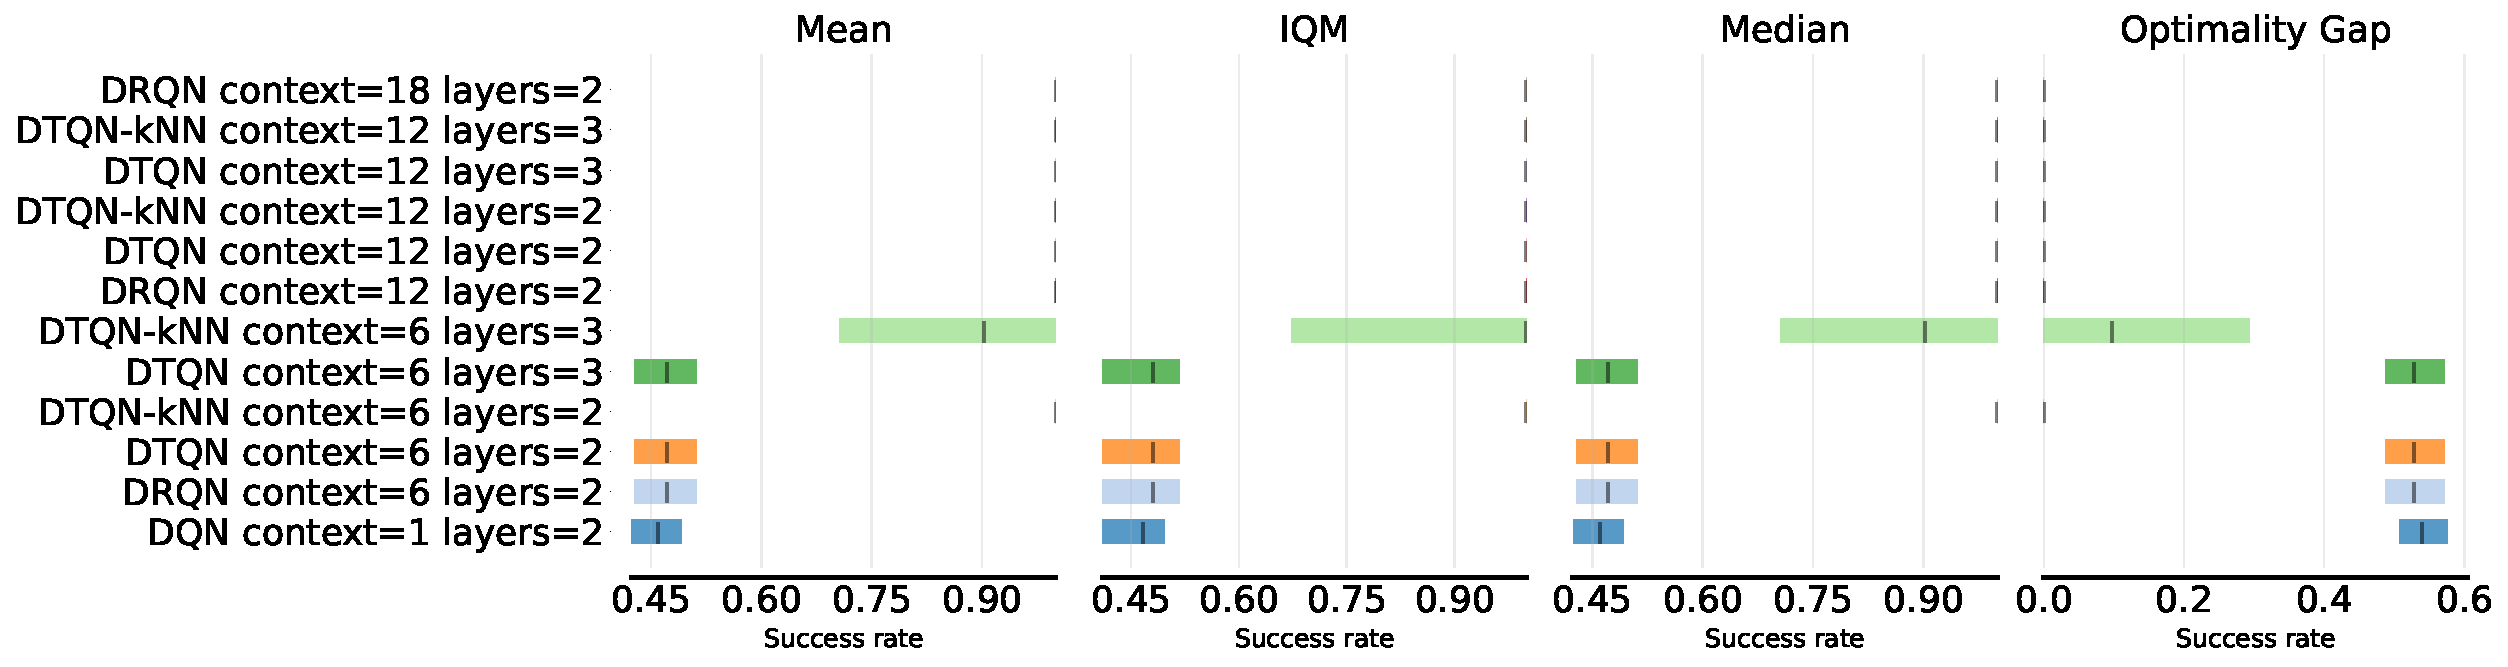
\includegraphics[width=\linewidth]{aggregate_metrics}
  \caption{Mean, interquartile mean (IQM), median and optimality gap of the final
    success rate, with 95\% stratified bootstrap confidence intervals.}
  \label{fig:aggregate-metrics}
\end{figure}

\begin{figure}[t]
  \centering
  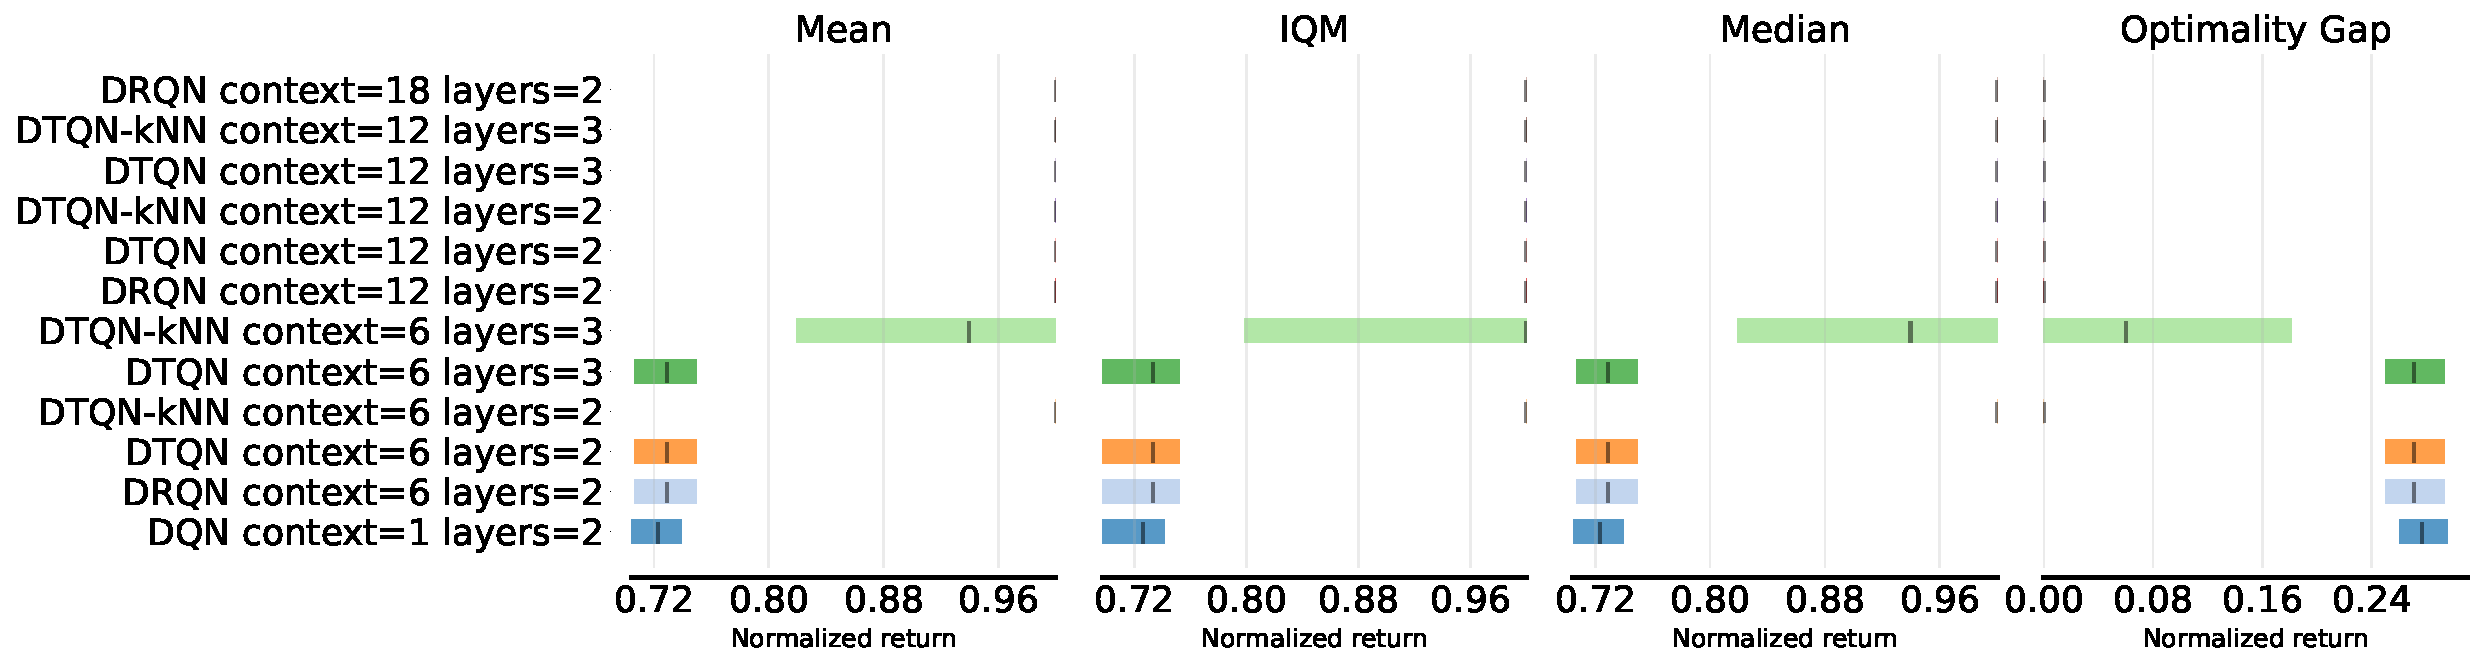
\includegraphics[width=\linewidth]{aggregate_metrics_return}
  \caption{Aggregate metrics of the final return, min-max normalized per task over
    all runs, with 95\% stratified bootstrap confidence intervals.}
  \label{fig:aggregate-metrics-return}
\end{figure}

\begin{figure}[t]
  \centering
  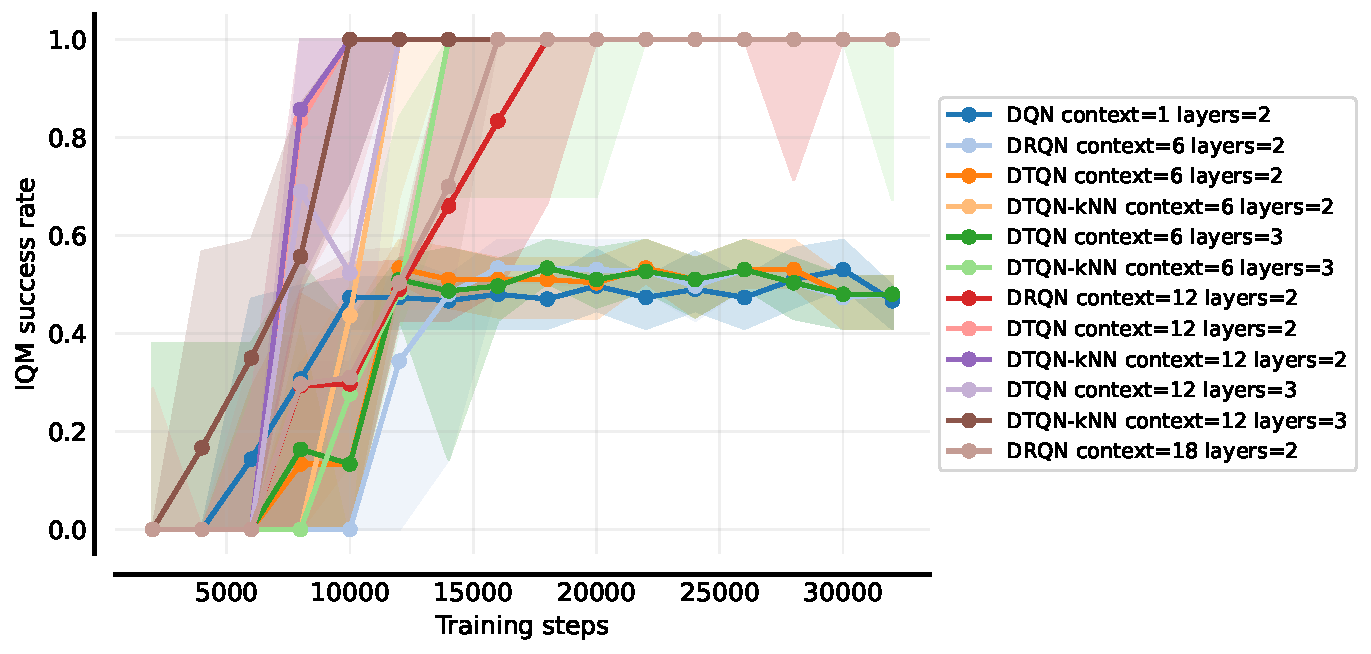
\includegraphics[width=\linewidth]{iqm_learning_curves}
  \caption{IQM success rate during training, with 95\% stratified bootstrap
    confidence bands.}
  \label{fig:iqm-learning-curves}
\end{figure}

\begin{figure}[t]
  \centering
  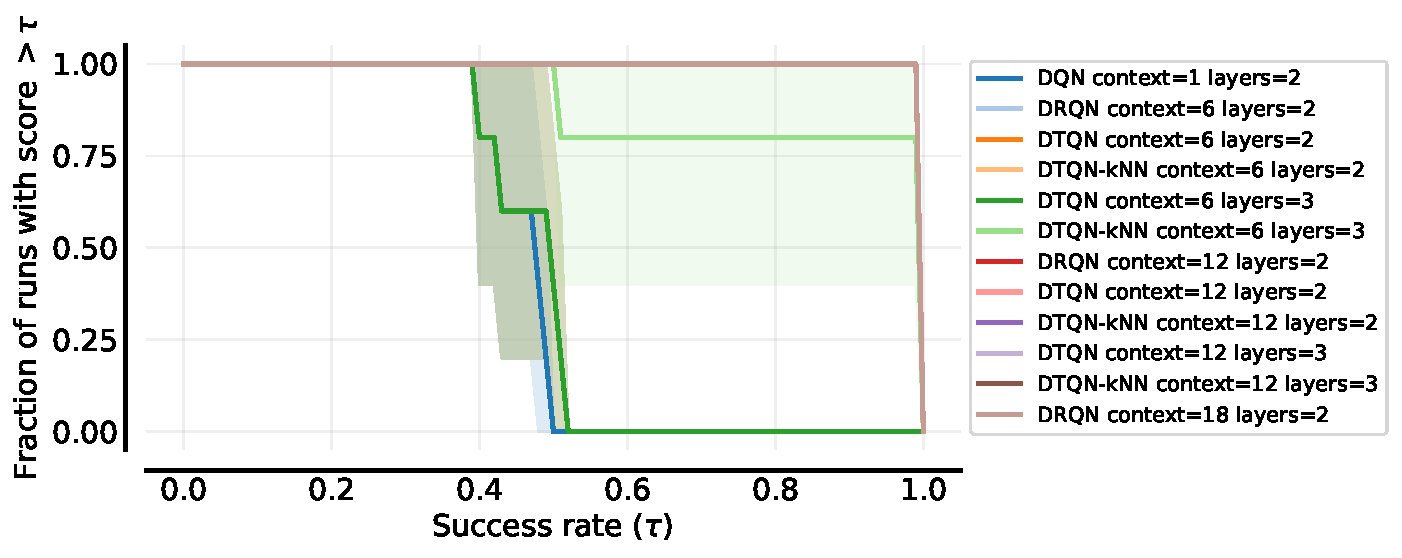
\includegraphics[width=\linewidth]{performance_profiles}
  \caption{Performance profiles: fraction of runs whose final success rate exceeds
    each threshold $\tau$, with 95\% confidence bands.}
  \label{fig:performance-profiles}
\end{figure}

\begin{figure}[t]
  \centering
  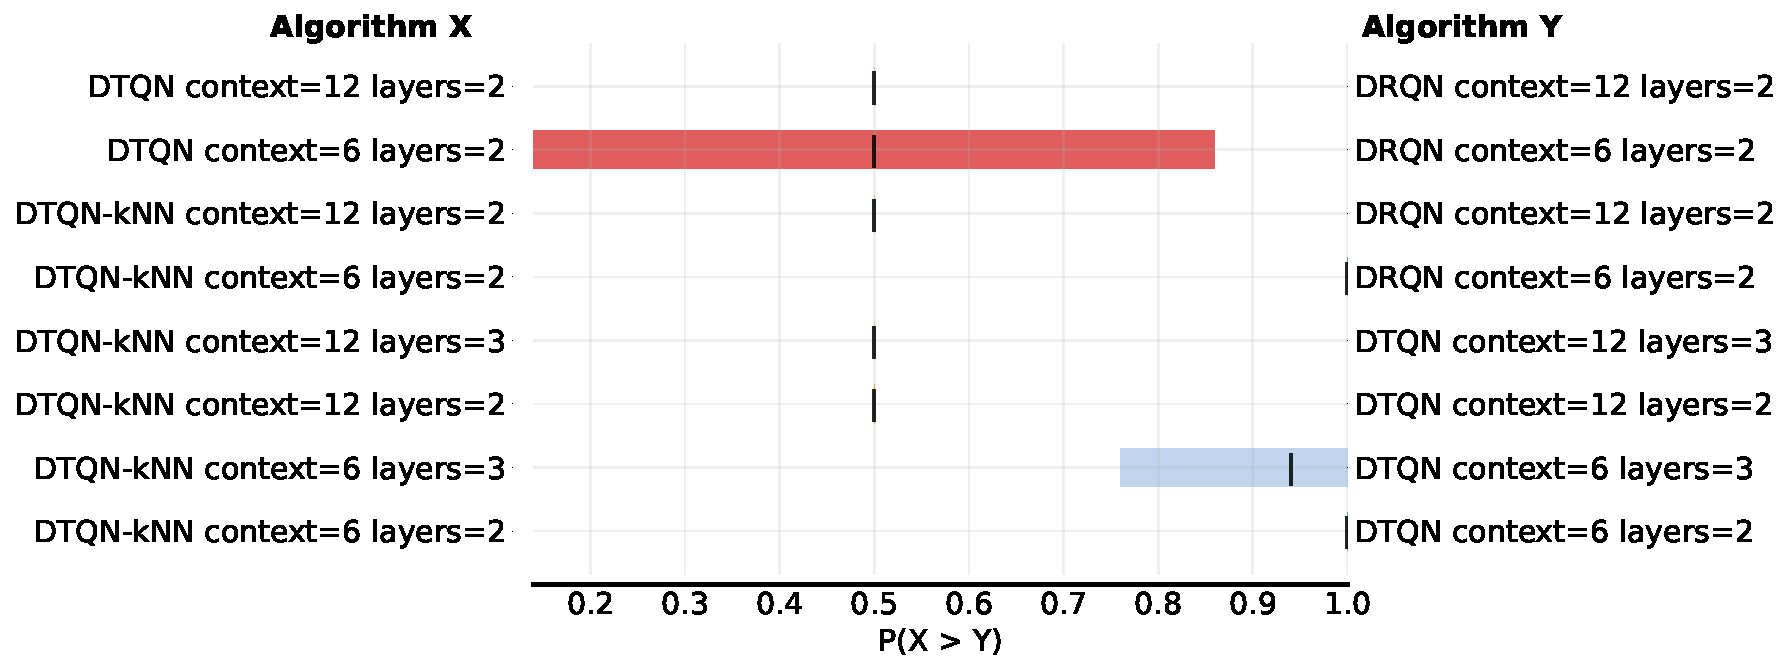
\includegraphics[width=0.8\linewidth]{probability_of_improvement}
  \caption{Probability of improvement of each candidate over its baseline with the
    same context length and number of layers, with 95\% confidence intervals.}
  \label{fig:probability-of-improvement}
\end{figure}
